
\documentclass[notes,11pt, aspectratio=169]{beamer}

\usepackage{pgfpages}
\usepackage{mdwlist}
% These slides also contain speaker notes. You can print just the slides,
% just the notes, or both, depending on the setting below. Comment out the want
% you want.
\setbeameroption{hide notes} % Only slide
%\setbeameroption{show only notes} % Only notes
%\setbeameroption{show notes on second screen=right} % Both

\usepackage{helvet}
\usepackage[default]{lato}
\usepackage{array}
\usepackage{tgbonum}
\usepackage[sfdefault]{FiraSans} %% option 'sfdefault' activates Fira Sans as the default text font
\usepackage[T1]{fontenc}
\renewcommand*\oldstylenums[1]{{\firaoldstyle #1}}

\usepackage{tikz}
\usepackage{verbatim}
\setbeamertemplate{note page}{\pagecolor{yellow!5}\insertnote}
\usetikzlibrary{positioning}
\usetikzlibrary{snakes}
\usetikzlibrary{calc}
\usetikzlibrary{arrows}
\usetikzlibrary{decorations.markings}
\usetikzlibrary{shapes.misc}
\usetikzlibrary{matrix,shapes,arrows,fit,tikzmark}
\usepackage{amsmath}
\usepackage{mathpazo}
\usepackage{hyperref}
\usepackage{lipsum}
\usepackage{multimedia}
\usepackage{graphicx}
\usepackage{multirow}
\usepackage{graphicx}
\usepackage{dcolumn}
\usepackage{bbm}
\newcolumntype{d}[0]{D{.}{.}{5}}

\usepackage{changepage}
\usepackage{appendixnumberbeamer}
\newcommand{\beginbackup}{
   \newcounter{framenumbervorappendix}
   \setcounter{framenumbervorappendix}{\value{framenumber}}
   \setbeamertemplate{footline}
   {
     \leavevmode%
     \hline
     box{%
       \begin{beamercolorbox}[wd=\paperwidth,ht=2.25ex,dp=1ex,right]{footlinecolor}%
%         \insertframenumber  \hspace*{2ex} 
       \end{beamercolorbox}}%
     \vskip0pt%
   }
 }
\newcommand{\backupend}{
   \addtocounter{framenumbervorappendix}{-\value{framenumber}}
   \addtocounter{framenumber}{\value{framenumbervorappendix}} 
}


\usepackage{graphicx}
\usepackage[space]{grffile}
\usepackage{booktabs}
\newcommand\independent{\protect\mathpalette{\protect\independenT}{\perp}}
\def\independenT#1#2{\mathrel{\rlap{$#1#2$}\mkern2mu{#1#2}}}
\DeclareMathOperator{\Supp}{Supp}

% These are my colors -- there are many like them, but these ones are mine.
\definecolor{blue}{RGB}{0,114,178}
\definecolor{red}{RGB}{213,94,0}
\definecolor{yellow}{RGB}{240,228,66}
\definecolor{green}{RGB}{0,158,115}

\hypersetup{
  colorlinks=false,
  linkbordercolor = {white},
  linkcolor = {blue}
}


%% I use a beige off white for my background
\definecolor{MyBackground}{RGB}{255,253,218}

%% Uncomment this if you want to change the background color to something else
%\setbeamercolor{background canvas}{bg=MyBackground}

%% Change the bg color to adjust your transition slide background color!
\newenvironment{transitionframe}{
  \setbeamercolor{background canvas}{bg=yellow}
  \begin{frame}}{
    \end{frame}
}

\setbeamercolor{frametitle}{fg=blue}
\setbeamercolor{title}{fg=black}
\setbeamertemplate{footline}[frame number]
\setbeamertemplate{navigation symbols}{} 
\setbeamertemplate{itemize items}{-}
\setbeamercolor{itemize item}{fg=blue}
\setbeamercolor{itemize subitem}{fg=blue}
\setbeamercolor{enumerate item}{fg=blue}
\setbeamercolor{enumerate subitem}{fg=blue}
\setbeamercolor{button}{bg=MyBackground,fg=blue,}



% If you like road maps, rather than having clutter at the top, have a roadmap show up at the end of each section 
% (and after your introduction)
% Uncomment this is if you want the roadmap!
% \AtBeginSection[]
% {
%    \begin{frame}
%        \frametitle{Roadmap of Talk}
%        \tableofcontents[currentsection]
%    \end{frame}
% }
\setbeamercolor{section in toc}{fg=blue}
\setbeamercolor{subsection in toc}{fg=red}
\setbeamersize{text margin left=1em,text margin right=1em} 

\newenvironment{wideitemize}{\itemize\addtolength{\itemsep}{10pt}}{\enditemize}

\usepackage{environ}
\NewEnviron{videoframe}[1]{
  \begin{frame}
    \vspace{-8pt}
    \begin{columns}[onlytextwidth, T] % align columns
      \begin{column}{.70\textwidth}
        \begin{minipage}[t][\textheight][t]
          {\dimexpr\textwidth}
          \vspace{8pt}
          \hspace{4pt} {\Large \sc \textcolor{blue}{#1}}
          \vspace{8pt}
          
          \BODY
        \end{minipage}
      \end{column}%
      \hfill%
      \begin{column}{.38\textwidth}
        \colorbox{green!20}{\begin{minipage}[t][1.2\textheight][t]
            {\dimexpr\textwidth}
            Face goes here
          \end{minipage}}
      \end{column}%
    \end{columns}
  \end{frame}
}

\title[]{\textcolor{blue}{Hierarchical models + Bayesian shrinkage}}
\author[PGP]{}
\institute[FRBNY]{\small{Paul Goldsmith-Pinkham}}
\date{\today}


\begin{document}

%%% TIKZ STUFF
\tikzset{   
        every picture/.style={remember picture,baseline},
        every node/.style={anchor=base,align=center,outer sep=1.5pt},
        every path/.style={thick},
        }
\newcommand\marktopleft[1]{%
    \tikz[overlay,remember picture] 
        \node (marker-#1-a) at (-.3em,.3em) {};%
}
\newcommand\markbottomright[2]{%
    \tikz[overlay,remember picture] 
        \node (marker-#1-b) at (0em,0em) {};%
}
\tikzstyle{every picture}+=[remember picture] 
\tikzstyle{mybox} =[draw=black, very thick, rectangle, inner sep=10pt, inner ysep=20pt]
\tikzstyle{fancytitle} =[draw=black,fill=red, text=white]
%%%% END TIKZ STUFF

% Title Slide
\begin{frame}
\maketitle

\end{frame}


\begin{frame}{Today's topic: hierarchical modeling + shrinkage}
  \begin{columns}[T] % align columns
    \begin{column}{.7\textwidth}
      \begin{wideitemize}
      \item Already touched on shrinkage in the context of lasso
        \begin{itemize}
        \item Today, we're going to provide a more general model
          structure for shrinkage and penalization
        \end{itemize}
      \item Going to be studying a framework for thinking about two (simultaneous) features of our estimates:
        \begin{itemize}
        \item Estimation uncertainty
        \item True heterogeneity
        \end{itemize}
      \item When considering two (or more) estimates, differences and
        variation in these estimates can be driven by either noise, or
        true variation
        \begin{itemize}
        \item Goal today is to give a framework for considering these
        \item Additional, highlight that there are improved methods
          that can be used for some estimands
        \end{itemize}
      \end{wideitemize}
    \end{column}%
  \hfill%
  \begin{column}{.4\textwidth}
  \end{column}
\end{columns}
\end{frame}


\begin{frame}{Motivation for Bayesian approaches}
  \begin{wideitemize}
  \item To motivate and give context to our discussion, will present the
    following four examples.
  \item These are very different types of problems, but will all
    hopefully be more accessible following our discussion today.
  \end{wideitemize}
\end{frame}
\begin{frame}{Four examples - (1) Microcredit + pooling}
  \begin{wideitemize}
  \item A set of experiments run in different locations, studying the
    efficiacy of microcredit on a variety of outcomes
    \begin{itemize}
    \item Meager (2019)
    \end{itemize}
  \item For every location $l$, we have a treatment, $T$,
    affecting our outcomes $Y$.
  \item We can use this to estimate $\hat{\tau}_{l}$, an unbiased
    estimate of the effect of microcredit in location $l$, $\tau_{l}$
    \begin{itemize}
    \item Note that these can be very different experiments
    \item This gives a set of estimates, $\boldsymbol{\hat{\tau}} = \{\hat{\tau}_{1},\ldots, \hat{\tau}_{L}\}$
    \end{itemize}
  \item What are things we might want to say about these?
    \begin{itemize}
    \item Are they similar to one another? If so, is that informative external validity?
    \item Are they different? Is that because of estimation error, or heterogeneity?
    \end{itemize}
  \item Could we improve on predictions more generally?
    \begin{itemize}
     \item Chetty and Hendren (2017), Angrist et al. (2017),
      Goldsmith-Pinkham, Pinkovskiy and Wallace (2021)
    \end{itemize}
  \end{wideitemize}
\end{frame}

\begin{frame}{Four examples - (2) Predictability and uncertainty}
  \begin{wideitemize}
  \item Excess stock returns (above some risk free rate) are
    predictable based on historical data (e.g. the dividend
    yield). How does this affect our willingness to invest in stocks,
    depending on our horizon?
    \begin{itemize}
    \item Barberis (2000)
    \end{itemize}
  \item Our returns in period $t$ are a predictable feature of lagged
    returns $r_{t-1}$ and other characteristics $x_{t-1}$ (plus some innovation):
    \begin{equation*}
      z_{t} = \alpha + x_{t-1}B +  \epsilon_{t},
    \end{equation*}
    where $z_{t} = (r_{t}, x_{t})$ and
    $\epsilon \sim \mathcal{N}(0,\Sigma)$ (e.g. a VAR)
  \item These VAR parameters ($\alpha, B, \Sigma$) are easily
    estimated using historical data
    \begin{itemize}
    \item We can use this to model predictions about future values of $r_{t+k}$
    \end{itemize}
  \item Riskiness in the investment will drive our decision in how much to invest
    \begin{itemize}
    \item But crucially, riskiness is not just a function of $\Sigma$
    \item The uncertainty of $\alpha$ and $B$ play an important role
    \end{itemize}
  \end{wideitemize}
\end{frame}


\begin{frame}{Four examples - (3) Estimation}
  \begin{wideitemize}
  \item Recall from demand models that choice modeling can be complex
    \begin{itemize}
    \item Important to allow for rich forms of choice substitution and
      preference heterogeneity
    \end{itemize}
  \item Imagine we want to model labor supply of Uber drivers (Chen et al. (2019))
    \begin{itemize}
    \item Specficially model the time-varying reservation wage for drivers
      $$w_{it}^{*} = \mu_{i}(t) + \epsilon_{it}$$
    \item $w_{it}^{*}$ unobserved, but we see the decision to work,
      and the expected wage at a given time
    \end{itemize}
  \item Crucially, a rich and flexible structure on $\epsilon_{it}$ is necessary, but makes things computationally complicated
    \begin{itemize}
    \item Analgous to the multivariate logit / probit problem
    \end{itemize}
  \item Can we use structure on the errors to make estimation feasible?
  \end{wideitemize}
\end{frame}

\begin{frame}{Four examples - (4) Multiple testing}
  \begin{wideitemize}
  \item One serious concern that has arisen is multiple testing issues in empirical analysis:
    \begin{itemize}
    \item ``Data mining'' a specification by running many regressions until a significant regression is achieved
    \end{itemize}
  \item This is particularly a concern in empirical asset pricing ( Harvey et al. (2016))
  \item Bayesian hierarchical models can jointly model the full set of
    empirical tests at the same time, and avoid any multiple testing
    complications 
    \begin{itemize}
    \item Jensen, Kelly and Pedersen (2022) use exactly this framework
      to study the replicability of empirical papers showing significant alpha from new factors 
    \end{itemize}
  \end{wideitemize}
\end{frame}

\begin{frame}{Bayes' rule and the Likelihood}
  \begin{wideitemize}
  \item Recall from our (and your previous classes') discussion of the
    likelihood, that for a given model of i.i.d. data $(Y_{i},X_{i})_{i=1}^{n}$ with model parameters $\theta$, we write down our likelihood:
    \begin{equation*}
      L(\theta) = \prod_{i=1}^{n}f_{\theta}(Y_{i} , X_{i}) 
    \end{equation*}
  \item But really, this is just the joint probability of the data -- e.g. $f(Y , X)$. If we are willing to be Bayesian, e.g., view the parameter $\theta$ as a random variable, we can even say $f(Y , X |  \theta)$
    \begin{itemize}
    \item Then, by Bayes' rule, we know we can write
      \begin{equation*}
        f(\theta | Y, X) = \frac{f(Y , X | \theta) \times p(\theta)}{f(Y,X)}
      \end{equation*}
    \end{itemize}
    \item Note that this can be written as
      \begin{equation*}
        f(\theta | Y, X) \propto f(Y,  X | \theta) \times p(\theta),
      \end{equation*}
      because the denominator will only rescale the probability
      distribution to ensure that it is well-defined (integrates to 1)
  \end{wideitemize}
\end{frame}

\begin{frame}{Bayes' Rule and the Likelihood}
      \begin{equation*}
        f(\theta | Y, X) \propto f(Y X| \theta) \times p(\theta),
      \end{equation*}
  \begin{wideitemize}
  \item $f(\theta | Y, X)$ is known as the posterior of $\theta$,
    while $p(\theta)$ is known as the prior. Tying this all together is
    the likliehood -- $f(Y, X | \theta)$
  \item This is a simple application of Bayes' rule. However, it adds
    two crucial features to the likelihood:
    \begin{itemize}
    \item The prior $p(\theta)$. Picking a parameter that maximizes
      $L(\theta) \times p(\theta)$ will give different estimators than
      just $L(\theta)$ except in special cases
    \item Distribution of $\theta$ in finite samples. Recall that
      inference for MLE estiamtes of $\theta$ rely on asymptotic
      approximations of Normality
    \end{itemize}
  \end{wideitemize}
\end{frame}


\begin{frame}{Simple Bernouilli example}
  \begin{wideitemize}
  \item Let's start with a very simple example. We are considering a
    dataset of successes and failures (denoted by $X_{i}$)
    \begin{itemize}
    \item This is a binomial, with total outcomes $n$ and total failures
      $\sum_{i}X_{i}$
    \item Failure rate is initially assumed to be identical $p$
    \end{itemize}
  \item We know our joint distribution:
    $$ f(X | p) = p^{\sum_{i}X_{i}}(1-p)^{n - \sum_{i}X_{i}}$$
  \item We could solve for the MLE of $p$ easily -- that gives us
    $\hat{p}_{MLE} = \sum_{i}X_{i} / n$
  \item What does our \emph{posterior} of $p$ look like, given the data?
    \begin{itemize}
    \item First neeed a prior -- let's assume it's uniform over (0,1)
    \end{itemize}
  \item Then, the posterior is
    $$ f(p | X) \propto f(X | p) \times 1  = p^{\sum_{i}X_{i}}(1-p)^{n - \sum_{i}X_{i}}$$
    \begin{itemize}
    \item This is a \emph{Beta} distribution with
      parameters $\alpha = \sum_{i}X_{i} + 1$ and
      $\beta = n - \sum_{i}X_{i} + 1$.
    \item Posterior mean of Beta dist? $\alpha / (\alpha + \beta)$
      Posterior mode? $\alpha - 1 / (\alpha + \beta - 2)$
    \end{itemize}
  \end{wideitemize}
\end{frame}

\begin{frame}{Simple Bernouilli example}
  \begin{wideitemize}
  \item Our prior was pretty uninformative / uninteresting
    \begin{itemize}
    \item We can use a \emph{conjugate} prior and get easily interpretable posteriors
    \item E.g. conjugate prior for Bernouilli is a Beta distribution
    \item Let's assume a Beta prior with $\alpha_{p} = 1$ and $\beta_{p} = 1$ (mean of 0.5)
    \end{itemize}
  \item Then, the posterior is
    $$ f(p | X) \propto p^{\sum_{i}X_{i} + \alpha_{p}}(1-p)^{n - \sum_{i}X_{i} + \beta_{p}}$$
%$
    \begin{itemize}
    \item This is a \emph{Beta} distribution with
      parameters $\alpha = \sum_{i}X_{i} + \alpha_{p} - 1$ and
      $\beta = n - \sum_{i}X_{i} + \beta_{p} - 1$.
    \end{itemize}
  \item Hence our prior shifts our posterior estimates, but as $n$
    gets large, our posterior will converge to the MLE
  \end{wideitemize}
\end{frame}


\begin{frame}{Simple Normal example}
  \begin{wideitemize}
  \item Now let's consider another example with Normal distributions instead
  \item We observe a set of observations $X_{i}$ which we assume come
    from a normal distribution, with unknown mean and known variance
    $\sigma^{2} = 1$
    \begin{itemize}
    \item Knowing the variance just makes our life easier and is not necessary in general
    \item Note that this is saying $X_{i} = \mu + \epsilon_{i}$, $\epsilon_{i} \sim \mathcal{N}(0, 1)$
    \end{itemize}
  \item Recall that we need a prior to any Bayesian analysis. Our only
    unknown parameter is $\mu$. What is our prior over this?
    \begin{itemize}
    \item The conjugate prior for a Normal mean is also Normal
    \item Let's assume a prior with mean zero, and variance 100
    \end{itemize}
  \item Hence, we construct our posterior as:
    $$ f(\mu | X) \propto f(X | \mu) \times p(\mu) \propto  \exp\left(-\sum_{i}\frac{(x_{i} - \mu)^{2}}{2 \sigma^{2}}\right) \times \exp\left(-\frac{(\mu - 0)^{2}}{2 \times 100}\right) $$
  \item The trick is to combine terms, and then drop out any that do
    not involve $\mu$. Then, complete the square.
  \end{wideitemize}
\end{frame}
\begin{frame}{Simple Normal example}
  \begin{wideitemize}
  \item We are left with
    \begin{align*}
      f(\mu | X) &\propto  \exp\left(\frac{(\mu - \mu_{post})^{2}}{2 \sigma_{post}^{2}}\right)\\
      \mu_{post}       &=  \frac{\sum_{i}x_{i}}{n + 1/100}\\
      \sigma^{2}_{post}       &=  \left(\frac{1}{100} + \frac{n}{1}\right)^{-1}
    \end{align*}
  \item In our setting, recall we had a prior at zero, with a large
    variance (so we really weren't very precise)
    \begin{itemize}
    \item As a consequence, our posterior mean is shrunk towards zero,
      but not by a lot
    \item If we make the prior more informative (smaller variance) or
      move the shrinkage point, that shifts both parameters
    \item Again, as the data gets large, the prior (should) matter less
    \end{itemize}
  \end{wideitemize}
  \end{frame}

\begin{frame}{Shrinkage with more structure}
  \begin{wideitemize}
  \item So far, our analysis focused on single parameter estimation
    \begin{itemize}
    \item Now let's consider a set of mean parameters that we're interested in across locations
    \item We're going to create hiearchichical structure on our parameters
    \end{itemize}
  \item Consider means across $l$ locations, where we observe
    observations within each location, and we model this as:
    \begin{align*}
      y_{il} &\sim \mathcal{N}(\mu_{l}, \sigma^{2})\\
      \mu_{l} &\sim \mathcal{N}(\mu, \eta^{2})
    \end{align*}
    (assuming $\sigma^{2}$ is known for simplicity)
  \item Note that we could write a simple version of this as:
    \begin{equation*}
      y_{il} = \mu + \underbrace{(\mu_{l} - \mu)}_{\text{Variation from heterogeneity}} + \underbrace{(y_{il} - \mu_{l})}_{\text{Sampling variation}}
    \end{equation*}
    where the two pieces on the right are random variables
  \end{wideitemize}
\end{frame}

\begin{frame}{Shrinkage with more structure}
    \begin{align*}
      y_{il} &\sim \mathcal{N}(\mu_{l}, \sigma^{2})\\
      \mu_{l} &\sim \mathcal{N}(\mu, \eta^{2})
    \end{align*}
  \begin{wideitemize}
  \item This is a hierarchical multivariate normal setting
    \begin{itemize}
    \item A simple version! For example, we could allow for
      correlation across locations, or within locations
    \item If you can dream it, you can try to estimate it
    \end{itemize}
  \item The key details:
    \begin{itemize}
    \item In this structure, like with the simple normal example, the
      estimate for $\mu_{l}$ will be shrunk towards the overall mean
      $\mu$. 
    \item This shrinkage will be a function of the relative variance $\sigma^{2}$ and $\eta^{2}$
    \item To do full Bayesian estimation here, recall that we need a
      prior for $\mu$ as well -- this would be specified by the
      researcher
      \begin{itemize}
      \item Implemnting this prior is the crucial distinction of going
        ``Full Bayes''
      \end{itemize}
    \end{itemize}
  \end{wideitemize}
\end{frame}

% \begin{frame}{Going fully hierarchical Bayes}
% \begin{center}
% \begin{tabular}{ccc}
%   \multicolumn{3}{c}{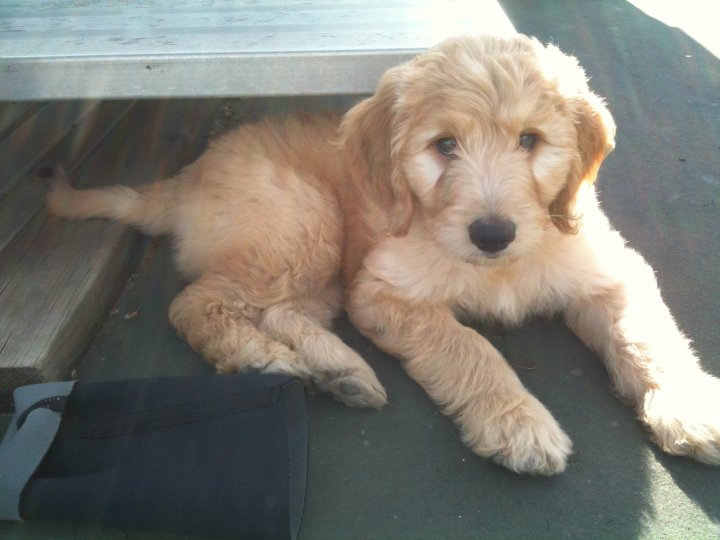
\includegraphics[width=0.3\linewidth]{images/bayes1.JPG}}\\
%   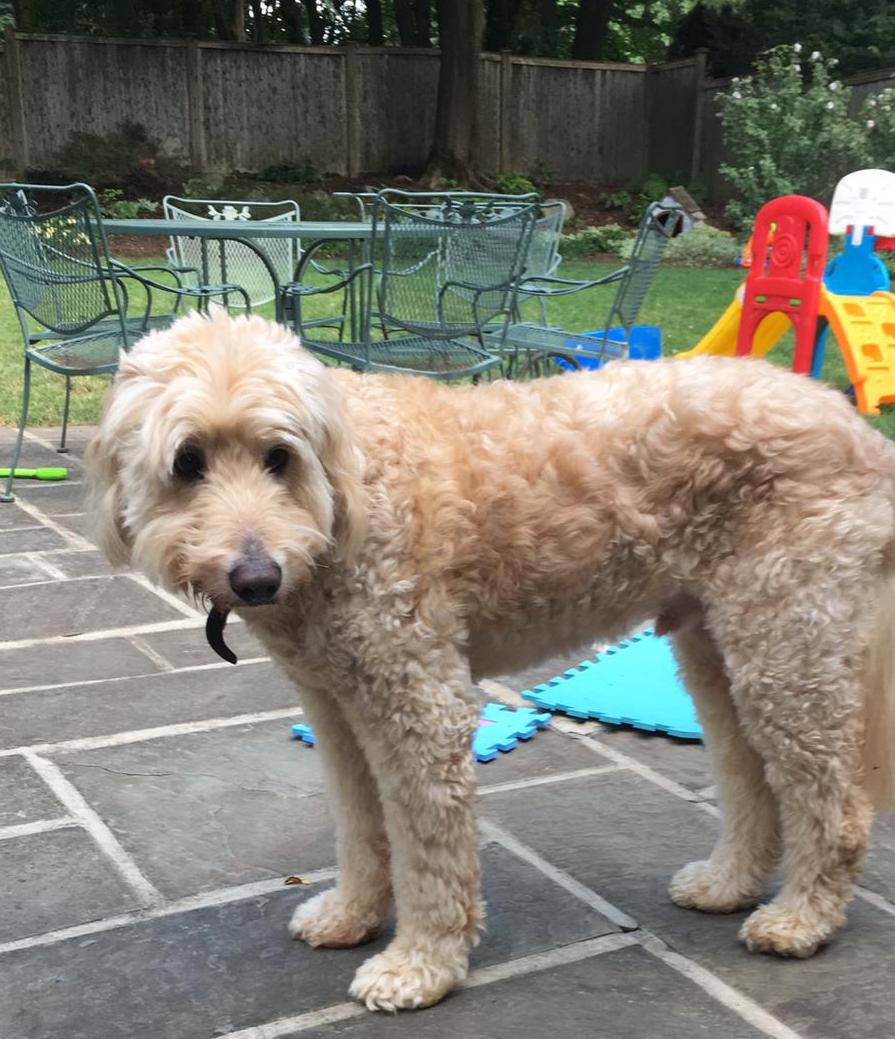
\includegraphics[width=0.24\linewidth]{images/bayes2.JPG} & 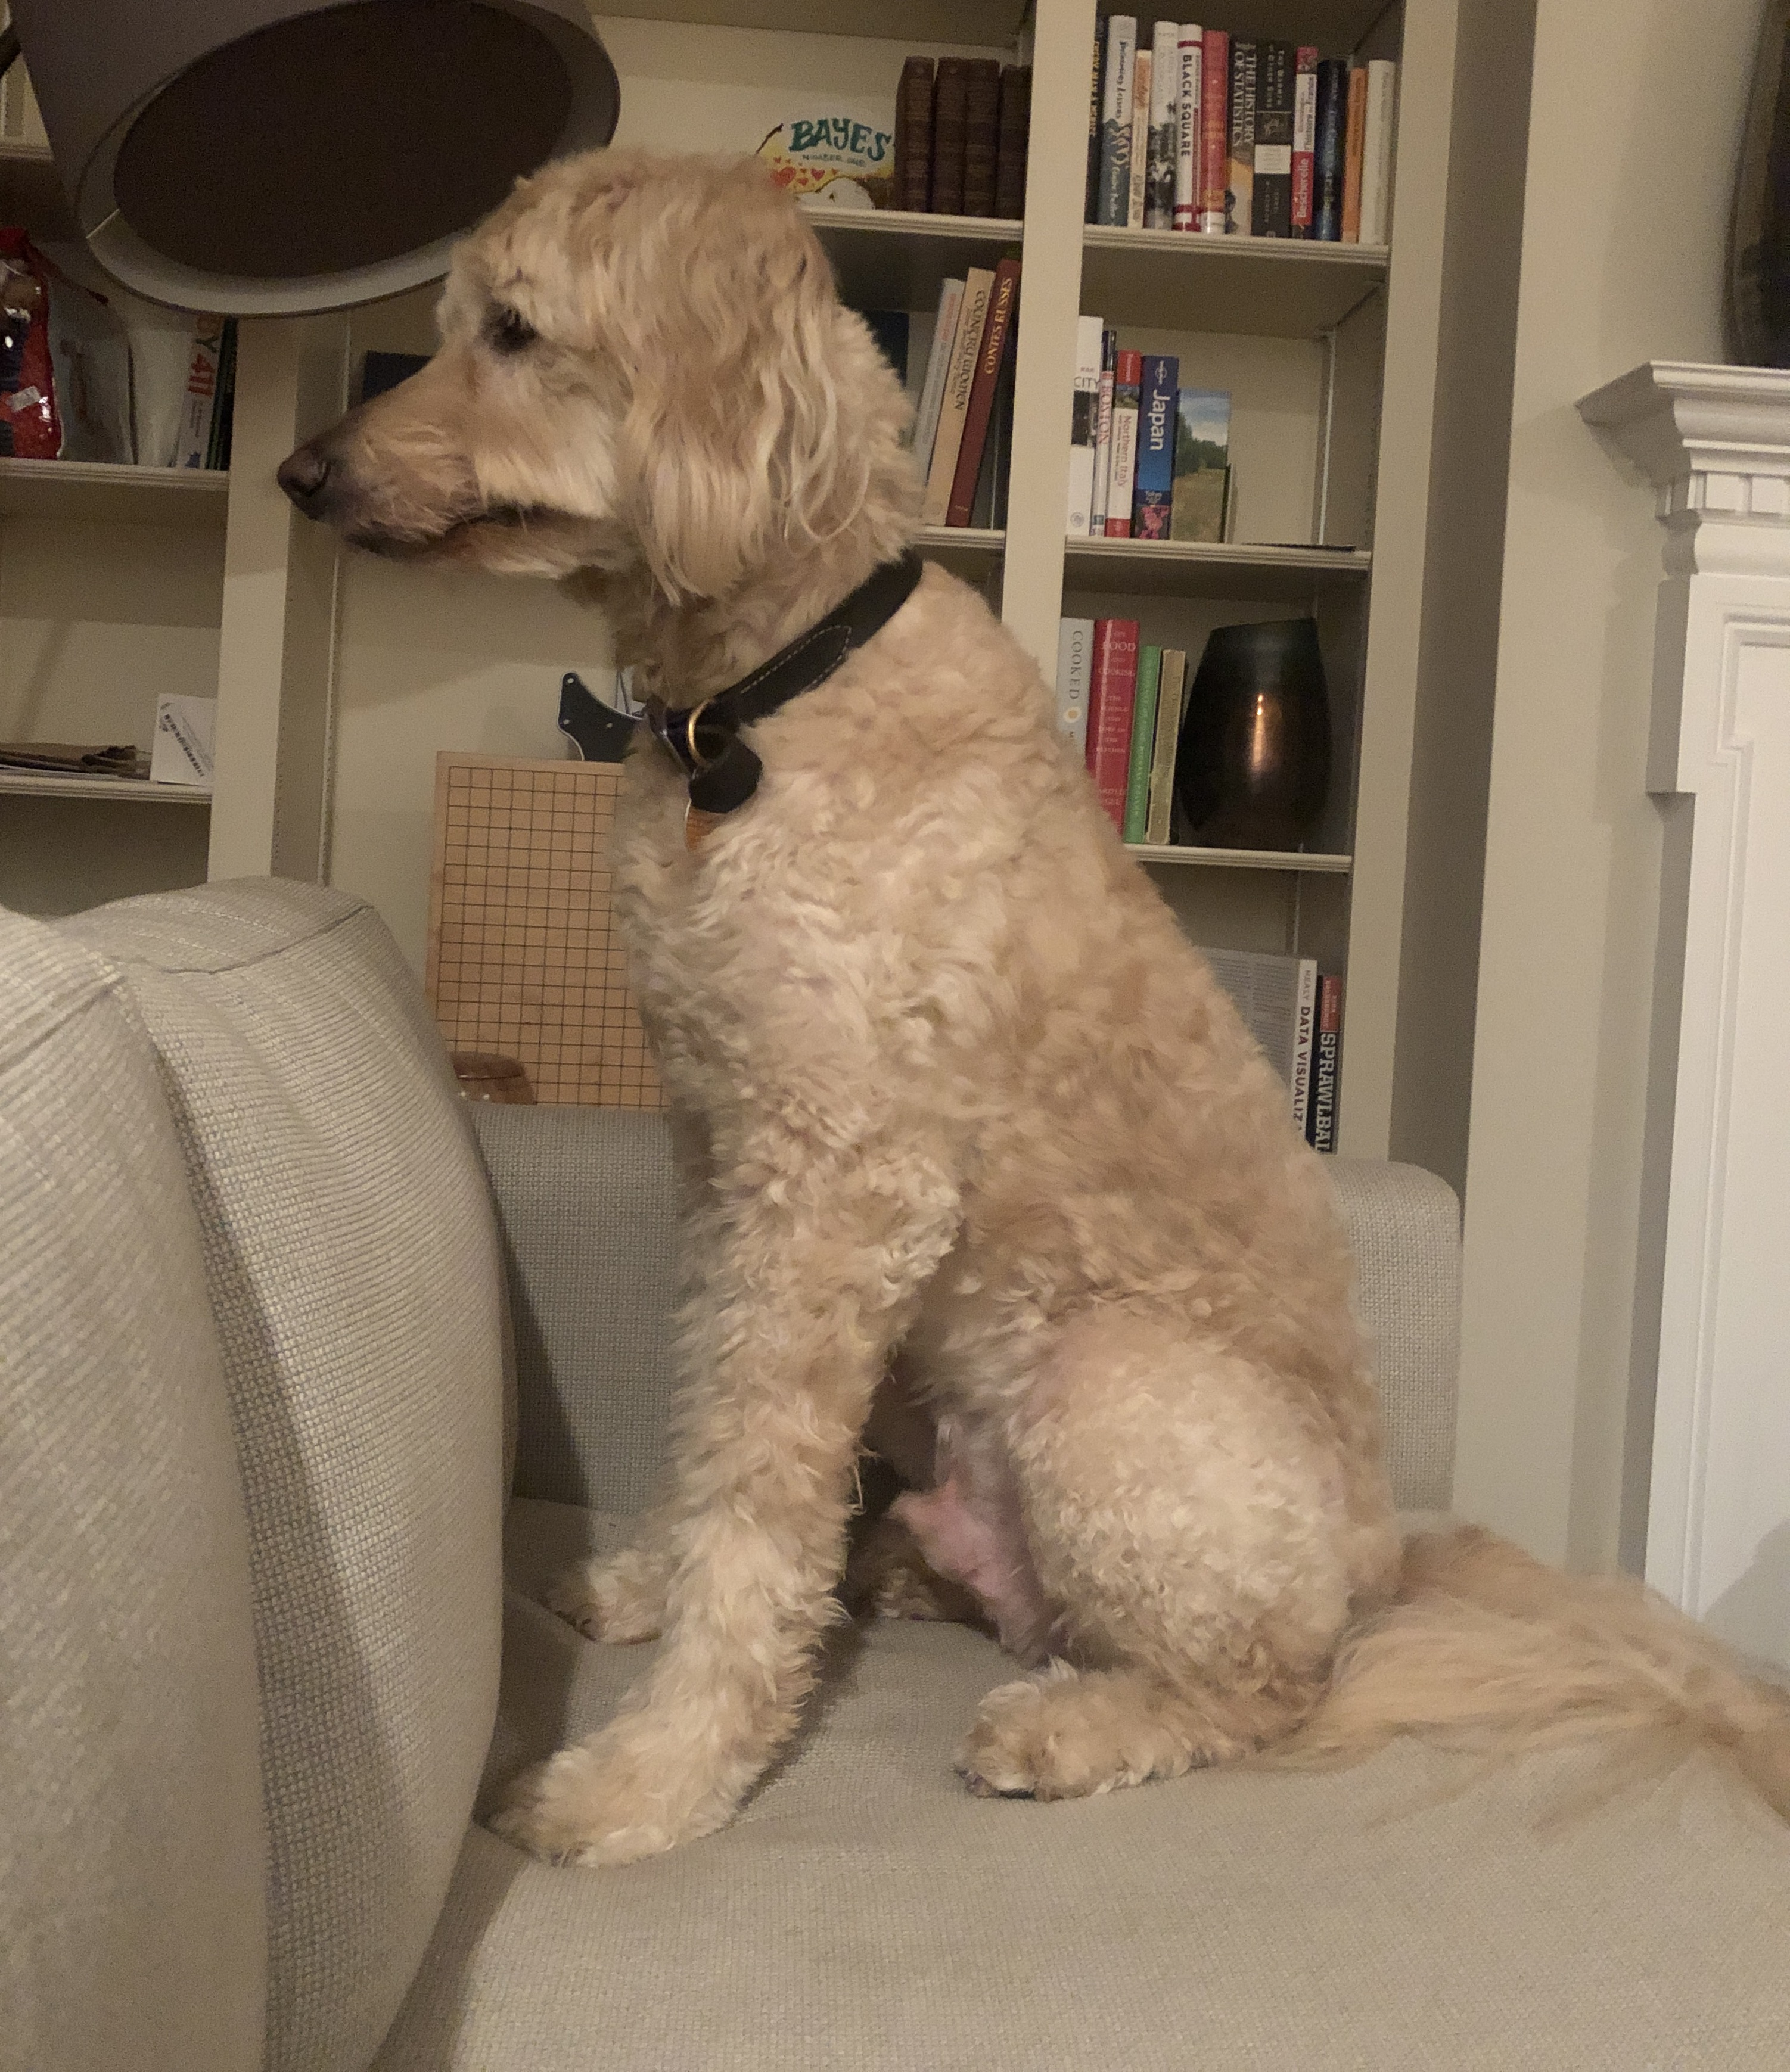
\includegraphics[width=0.24\linewidth]{images/bayes3.JPG} & 
\includegraphics[width=0.24\linewidth]{images/bayes4.JPG}\\
% \end{tabular}
% \end{center}
% \end{frame}


\begin{frame}{Why does adding this structure help?}
  \begin{wideitemize}
  \item Why would we want to add more structure in this way?
  \item Many potential reasons. A sample:
    \begin{enumerate}
    \item Allow for shrinkage that accounts for covariates (Meager study).
      \begin{itemize}
      \item Not only does this allow for shrinkage, but we can
        diagnose heterogeneity
      \end{itemize}
    \item We can estimate posterior distributions of estimates, and
      consider predictive distributions of outcomes (Barberis study)
      \begin{itemize}
      \item We have estimates of $p(\theta | X)$ (posterior), but can
        also estimate $p(X_{new} | X)$ (posterior predictive)
      \end{itemize}
    \item We can estimate much more complicated statistical systems using computational techniques
      \begin{itemize}
      \item E.g. complicated demand and supply systems! (Chen et al. (2019))
      \item Let's discuss this next
      \end{itemize}
    \end{enumerate}
  \end{wideitemize}
\end{frame}

\begin{frame}{Estimation of posterior using MCMC methods}
  \begin{wideitemize}
  \item So far, much of what we have discussed in these hierachical
    models were either simple (e.g. assumed known variances) or
    conjugate (very restrictive assumptions on parametrization)
  \item None of this is necessary -- Bayes' rule is well-defined
    irrespective of the parameterization choices, and $\theta$ can include many terms:
    \begin{equation*}
      p(\theta | X) \propto f(X | \theta) p(\theta)
    \end{equation*}
  \item The question, of course, is that if an analytic solution does
    not fall out as in our examples above, how does one generate a
    posterior distribution for $\theta$?
  \item Key insight -- we want to generate a chain of estimates
    $\theta_{0}, \theta_{1}, \ldots,$ such that after sufficiently
    large $k$ , the estimates $\theta_{k}, \ldots$ are random draws
    from the posterior of $\theta$.
  \item E.g. consider the challenge in the Bernouilli example
    \begin{itemize}
    \item If I did not know the posterior parameters for the distribution (and the general form of the parameteric model), how do I algorithmically generate draws of $\theta$ such that they will line up?
    \end{itemize}
  \end{wideitemize}
\end{frame}

\begin{frame}{Estimation using Hamiltonian Monte Carlo (hybrid MCMC)}
  \begin{columns}[T] % align columns
    \begin{column}{.7\textwidth}
  \begin{wideitemize}
  \item Beyond scope of this course, but intuitively the problem of
    searching over this space is just as challenging as our
    discusssions of finding MLEs using numerical methods
  \item When I learned all of this in 2005, Gibbs Sampler and
    Metropolis-Hastings algorithms were the default approaches
    \begin{itemize}
    \item However, this is no longer the case! (Betancourt + Girolami
      (2013))
    \end{itemize}
  \item One of the fastest algorithms to use now is known as
    Hamiltonian Monte Carlo
    \begin{itemize}
    \item This method is much more complicated / challenging to implement that Gibbs or MH
    \item But, open source community has solved this problem through \textit{Stan} (RStan)
    \item If you are going this route, use Stan
    \end{itemize}
  \end{wideitemize}
\end{column}
\begin{column}{0.3\textwidth}
  
\includegraphics[width=\linewidth]{images/stan.png}
\end{column}
\end{columns}
\end{frame}

\begin{frame}{Downsides of Full Bayes}
  \begin{wideitemize}
  \item  What's the ``cost'' of all this?
  \item  In most cases, it's the parameterization.
  \item  We're typically quite uncomfortable with doing this
  \item e.g. consider the linear regression model -- how do you want
    to parametrize the error terms? Can we approximate ``robust'' se?
    It's semi-parametric!
  \item Potential solutions?
    \begin{itemize}
    \item Try to flexibly model the covariance structure
    \item Assume the asymptotic distribution of the parameters
    \end{itemize}
  \item The other ``downside'' -- uncomfortable with priors
    \begin{itemize}
    \item How do we know what to shrink to? Doesn't this create bias?
    \end{itemize}
  \end{wideitemize}
\end{frame}

\begin{frame}{Middle ground}
  \begin{wideitemize}
  \item If these are issues you have, there are middle ground solutions
  \item First, recall that much of the time, we assume our
    \emph{estimates} are normal (that's how we do inference --
    asymptotic normality)
    \begin{itemize}
    \item Classic result from Rubin (1981)
    \end{itemize}
  \item We can just consider parameters
    \begin{align*}
      \hat{\tau}_{l} &\sim \mathcal{N}(\tau_{l}, \hat{se}_{l}^{2})\\
      \tau_{l} &\sim \mathcal{N}(\tau, \sigma_{\tau}^{2})
    \end{align*}
  \item Now we just need a prior on $\tau$ and $\sigma_{\tau}^{2}$,
    and we can do full Bayes!
    \begin{itemize}
    \item But we didn't assume anything about the DGP of the outcomes
      -- we just focused on the normality of the estimates (and
      assumed unbiasedness)
    \end{itemize}
  \item So the only ``new'' thing we're doing is assuming priors (but
    ignoring all other data)
    \begin{itemize}
    \item How should we pick priors?
    \end{itemize}
  \end{wideitemize}
\end{frame}

\begin{frame}{Cheating on priors with Empirical Bayes}
  \begin{wideitemize}
  \item The problem is we don't know what prior to pick, a lot of the
    time. E.g., what should we shrink towards?
  \item The empirical Bayes approach suggests that the ``traditional'' estimator (e.g. the MLE) is good enough
    \begin{itemize}
    \item Intuitively -- shrink the values towards the overall mean
    \end{itemize}
  \item   This isn't really Bayesian but it seems to work -- ignores
  variability in this estimate
  \end{wideitemize}
\end{frame}


\begin{frame}{When can this be useful? Goldsmith-Pinkham et al. (2021)}
  \begin{columns}[T] % align columns
    \begin{column}{.5\textwidth}
  \begin{wideitemize}
  \item<1-> Paper studying Medicare impact on health insurance and credit outcomes
    \begin{itemize}
    \item We use Regression Discontinuity (RD), but just assume we
      have correctly estimated causal effects of Medicare in each
      location $\hat{\tau}_{l}$
    \end{itemize}
  \item<1-> These estimates are \emph{noisy}
  \item<2-> Simple approach: shrink these estimates towards the overall
    mean of our estimates, weighted by how noisy these estimates are
  \item<3-> This has substantial impact -- makes our estimates more precise, but also create bias for the very noisy estimates    
  \end{wideitemize}
\end{column}
\begin{column}{0.5\textwidth}
  \only<1>{  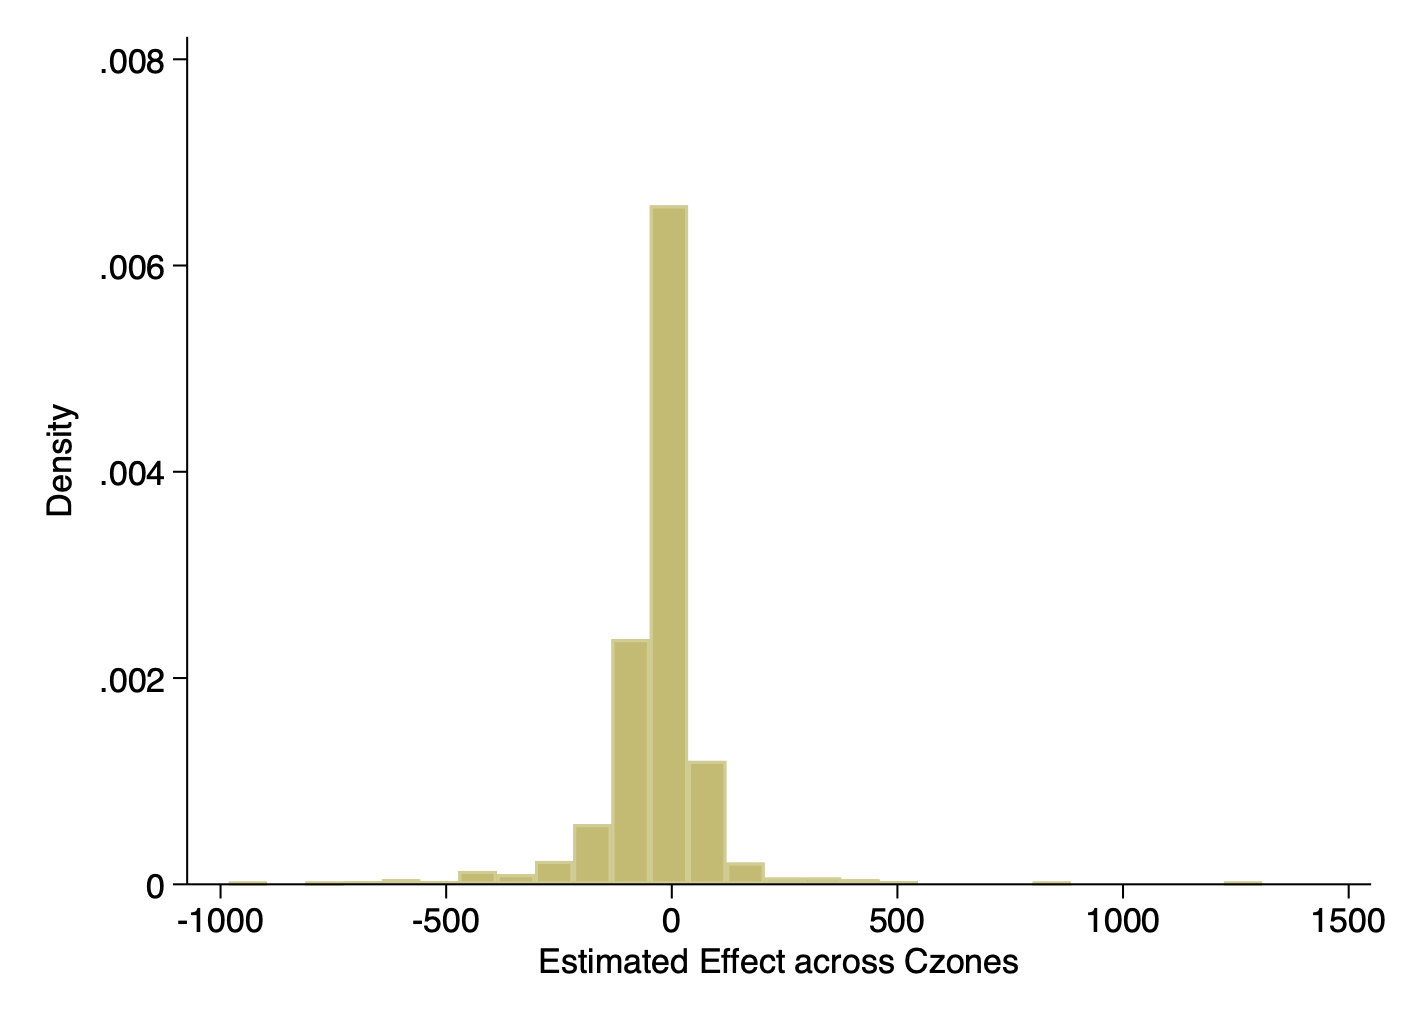
\includegraphics[width=\linewidth]{images/gpw1.png}}
  \only<2>{  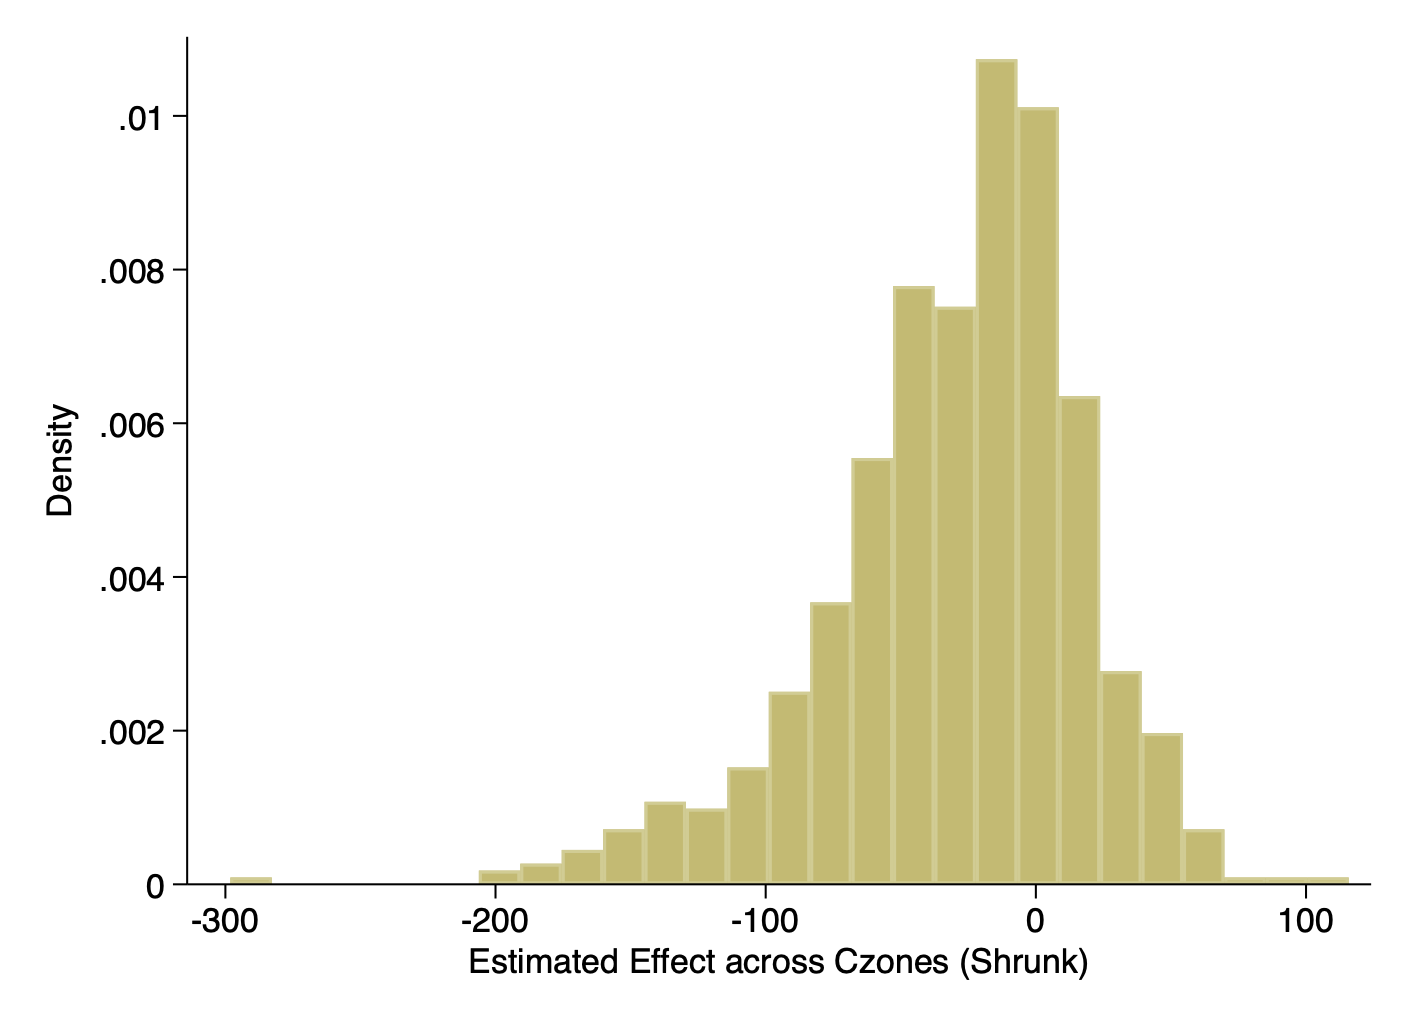
\includegraphics[width=\linewidth]{images/gpw2.png}}
  \only<3>{  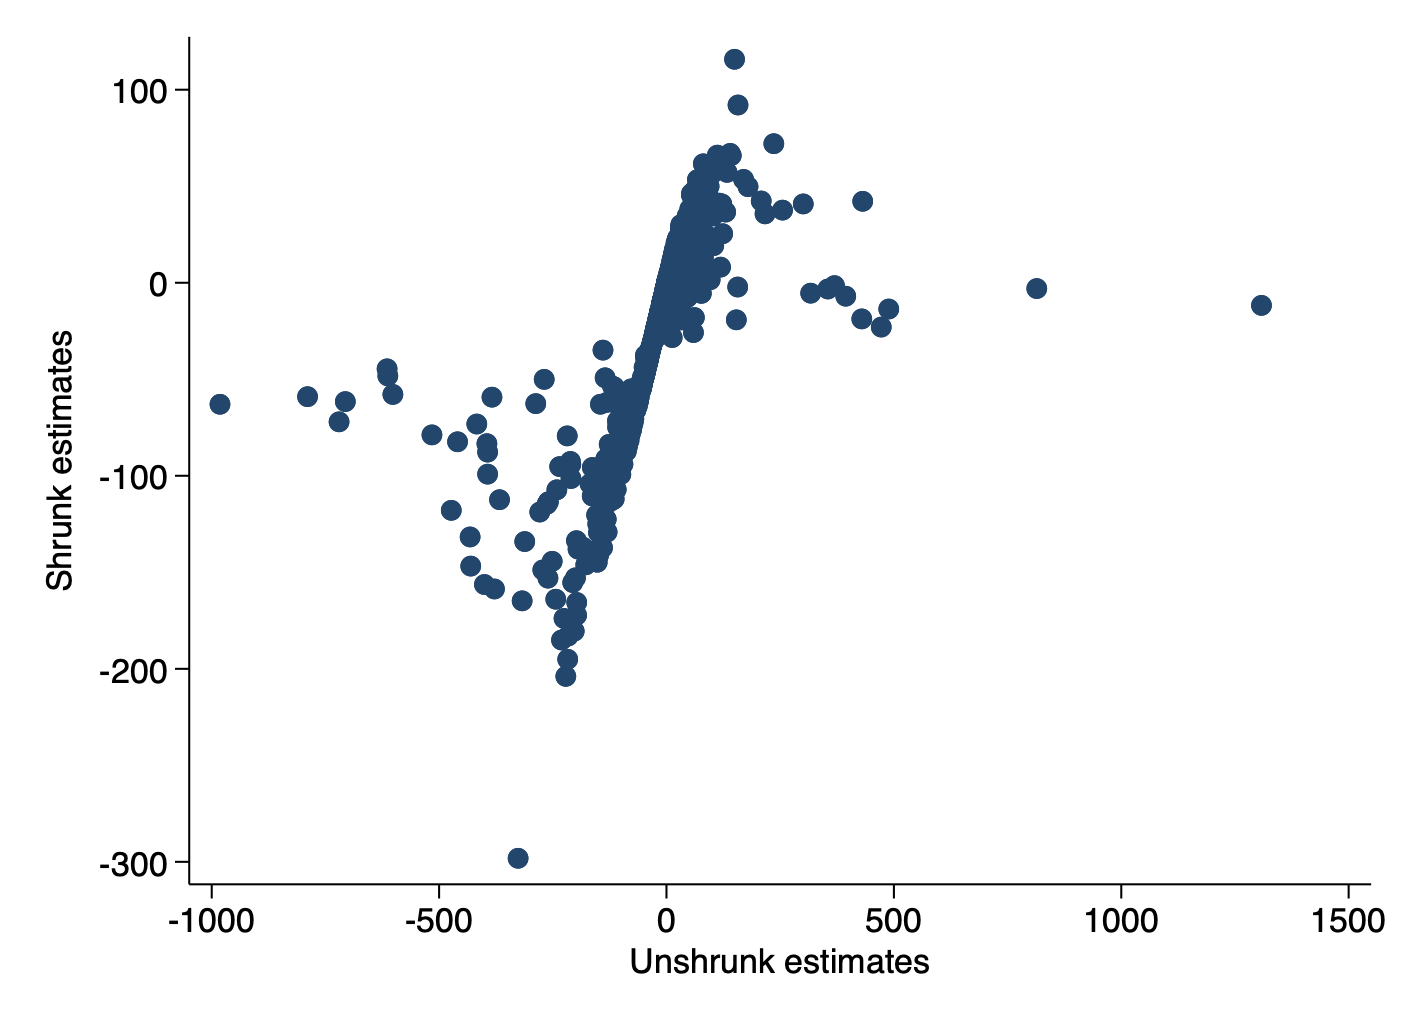
\includegraphics[width=\linewidth]{images/gpw3.png}}  
\end{column}
\end{columns}
\end{frame}

\begin{frame}{The shrinkage tradeoff}
  \begin{wideitemize}
  \item Remember the key reason why shrinkage is so effective:
    improvements on mean squared error are gained by increasing bias
  \item The ``shrunk'' estimates have some bias introduced in order to
    massive reduce their noise
  \item In economics, we've traditionally worried about unbiasedness a
    lot
    \begin{itemize}
    \item Important to identify what issues this can create
    \item If something is so noisy that it's not informative, a small
      amount of bias can be very useful
    \item Especially with prediction problems!
    \end{itemize}
  \item If we are trying to do prediction, forecast error (e.g. MSE)
    is typically much more important than unbiasedness
  \end{wideitemize}
\end{frame}

\begin{frame}{Having this structure gives intuition in many other settings}
  \begin{columns}[T] % align columns
    \begin{column}{.5\textwidth}
  \begin{wideitemize}
  \item This comes back to Lasso shrinkage
    \begin{itemize}
    \item Lasso can be viewed as a Laplace prior on the beta in our regression methods
    \end{itemize}
  \item Other regularization methods (e.g. ridge) use a less
    sharp-peaked prior (such as ridge, which is a Gaussian)
    \begin{align*}
      p(\beta | Y, X) &\propto f(Y,X | \beta, \sigma^{2}_{\epsilon}) p(\beta)\\
      \min_{\beta} \;& n^{-1}\sum_{i=1}^{n}(Y_{i} - X_{i}\beta)^{2} + \lambda \sum_{k=1}^{p}|\beta_{k}|
    \end{align*}
  \item Hence, the reasons behind Bayesian methods also motivate
    regularization methods and vice versa
  \end{wideitemize}
\end{column}
\begin{column}{0.5\textwidth}
  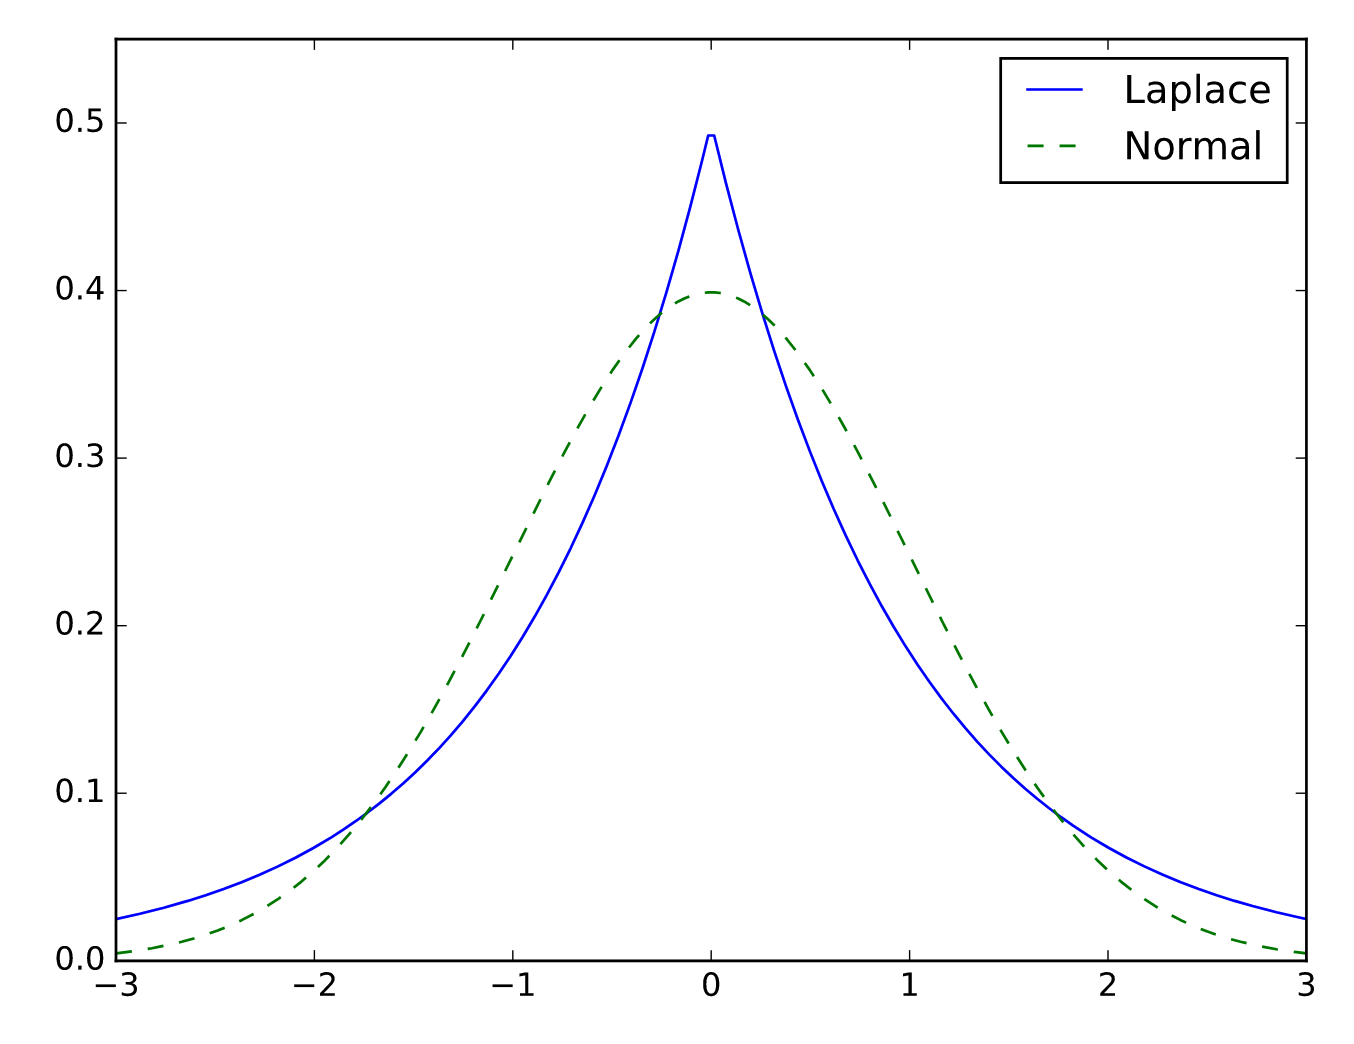
\includegraphics[width=\linewidth]{images/normal_laplace.png}
\end{column}
\end{columns}
  
\end{frame}



\begin{frame}{Conclude (before examples)}
  \begin{wideitemize}
  \item Adding structure can be very powerful, and is computationaly much easier to do now
  \item These techniques are widely applicable
    \begin{itemize}
    \item Finance, IO, labor, public
    \end{itemize}
  \item More generally, however, understanding how different methods
    incorporate shrinkage is valuable
  \item Decision tree for how to use these methods is non-obvious but for me, fall into three categories:
    \begin{enumerate}
    \item I have many noisy estimates, and I want to exploit their
      joint info (at minimum by regressing towards their average)
    \item I have a complicated statistical problem that I need to
      generate an underlying distribution from
    \item I need to predict outcomes incorporating estimated parameter
      uncertainty
    \end{enumerate}
\item You should consider Bayesian methods in this setting!
  \end{wideitemize}
 
\end{frame}

\begin{frame}{Example papers!}
  \begin{wideitemize}
  \item Meager (2017)
  \item Angrist et al. (2017)
  \item Johannes, Lochstoer and Mou (2016)
  \item Cohen and Einav (2007)
  \item Chinco et al. (2021)
  \item Athey et al. (2018)
    \item Mackey et al. (2015)
  \end{wideitemize}
  
\end{frame}

\end{document}